%タイトル
\begin{frame}
   \begin{center}
    \huge{子どもIT未来塾}
    \vspace{20pt}
	   {\huge 第7回}\\
	   {\huge ネットワークについて\\学ぼう}\\
    \vspace{24pt}
    \large{佐藤 雅俊}\\
    \vspace{10pt}
    \large{\the\year 年 8月25日}
  \end{center}
\end{frame}


\begin{frame}
	\frametitle{今回の授業について ~~~\raisebox{-3mm}{
\includegraphics[width=0.06\textwidth]{./slide07-img/raspberry.png}}}
		
 	% \frametitle{今回の授業について }

        \begin{description}
			\item[目標] ~\\
				\begin{itemize}\small
					\item ネチケットを知ろう
					\item ネットワークについて学ぼう
					\item CGIを使いこなそう
				\end{itemize}

			\item[授業の進め方]~\\
				\begin{itemize}\small
					\item 重要なことを先生が説明します
					\item スライドに示すページを開こう
					\item 例題・問題をすぐやろう\\
						やった問題にシールを貼ろう
				\end{itemize}
		\end{description}
		\vfill
		わからないことは、放っておかず、すぐにTAに聞きましょう
\end{frame}







\begin{frame}[fragile]
    \frametitle{ネチケットについて知ろう\\テキスト P.\pageref{1:P:Netiquette}~~~\raisebox{-3mm}{
\includegraphics[width=0.06\textwidth]{./slide07-img/raspberry.png}}}
    % \frametitle{ネチケットについて知ろう}
    インターネット上にもマナー、ルールがあります。ネット上のマナーのことを「ネチケット」といいます。
            \begin{itemize}\small
                \item 何も考えずにネットを利用すると、気づかないうちに犯罪者になってしまったり、犯罪にまきこまれたりします。
                \item 他人に迷惑をかけないことに加えて、ネチケットを守らない人から自分を守るために理解をしましょう。
            \end{itemize}
            \vfill
\end{frame}

\begin{frame}[fragile]
	\frametitle{ネチケットについて知ろう\\テキスト P.\pageref{1:P:Netiquette}~~~\raisebox{-3mm}{
\includegraphics[width=0.06\textwidth]{./slide07-img/raspberry.png}}}
    % \frametitle{ネチケットについて知ろう}

    \large\textbf{誰かが作ったものを勝手に使わない}
            \begin{itemize}\small
                \item 誰かが作ったものや情報には著作権というものがあり、法律で勝手に使うことは禁止されています。
                \item ただし、著作権は個人で楽しむものや、出典を明らかにして引用することは認められています。
            \end{itemize}
            \vfill
            
			\begin{minipage}{\textwidth}
                {\upshape
                  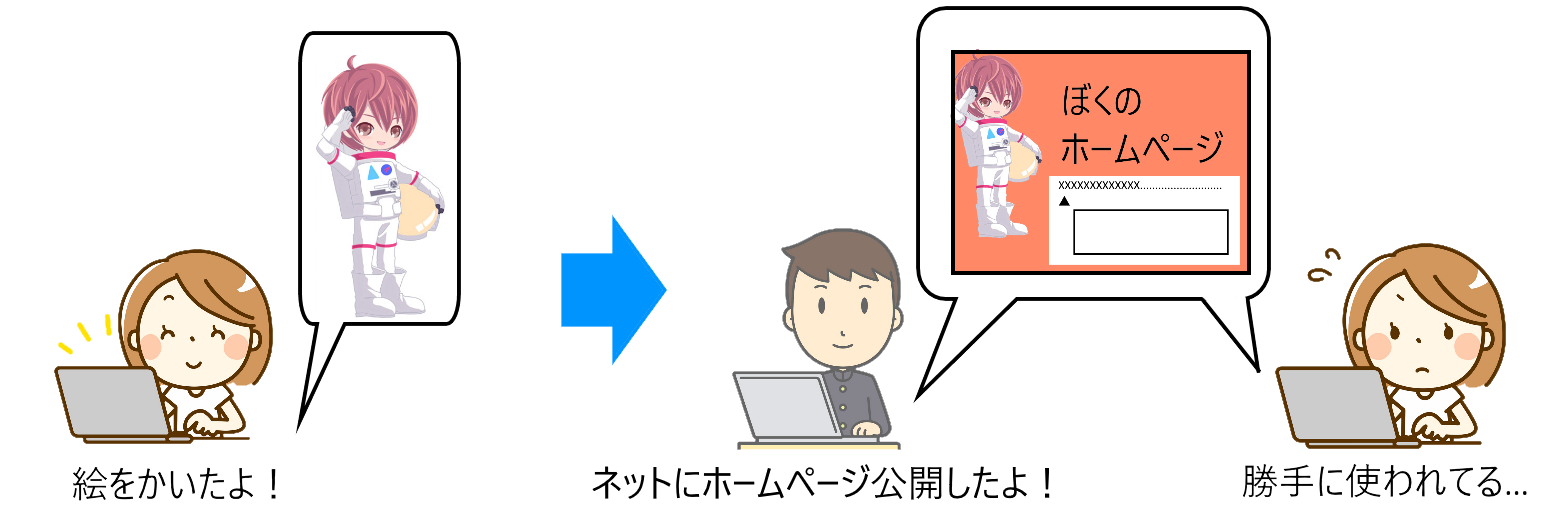
\includegraphics[width=\textwidth]{slide07-img/slide07-img001.png}}
            \end{minipage}
\end{frame}

\begin{frame}[fragile]
    \frametitle{ネチケットについて知ろう\\テキスト P.\pageref{1:P:Netiquette}~~~\raisebox{-3mm}{
\includegraphics[width=0.06\textwidth]{./slide07-img/raspberry.png}}}
    % \frametitle{ネチケットについて知ろう}
    % \large\textbf{人を傷つけることや、迷惑になることはやめる}
    \textbf{人を傷つけることや、迷惑になることはやめる}
            \begin{itemize}\small
                \item インターネットは自分以外の人も使っています。
                \item 自分勝手なことや悪い言葉を使ってばかりいると人を傷つけたり、不快に思われて犯罪に巻き込まれたり、訴えられる可能性もあります。
            \end{itemize}
            \vfill
            
			\begin{minipage}{0.7\textwidth}
                {\upshape
                  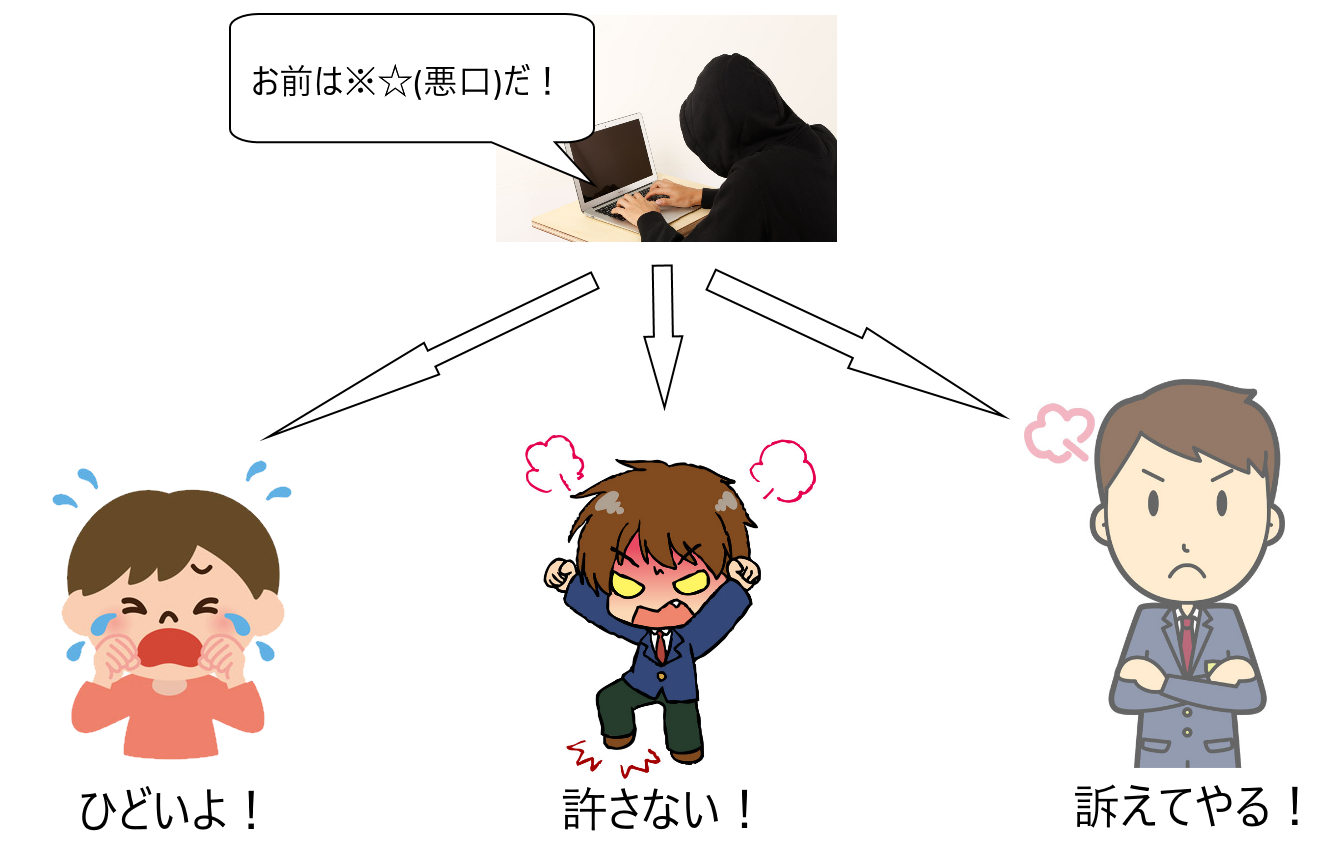
\includegraphics[scale=0.2]{slide07-img/slide07-img004.png}}
            \end{minipage}
\end{frame}

\begin{frame}[fragile]
    \frametitle{ネチケットについて知ろう\\テキスト P.\pageref{1:P:Netiquette}~~~\raisebox{-3mm}{
\includegraphics[width=0.06\textwidth]{./slide07-img/raspberry.png}}}
    % \frametitle{ネチケットについて知ろう}
    \large\textbf{他のひとたちが困らない文字情報を使う}
            \begin{itemize}\small
                \item ネットワークを使っている人たちはみんな同じものを使っているとは限りません。使って
                いる機種が、PC だったり、スマートフォンだったり、ラズベリーパイだったりします。
                \item 機種によっては、絵文字や特殊文字が見えなくなることが考えられます。                
            \end{itemize}
            \vfill
            
			\begin{minipage}{\textwidth}
                {\upshape
                  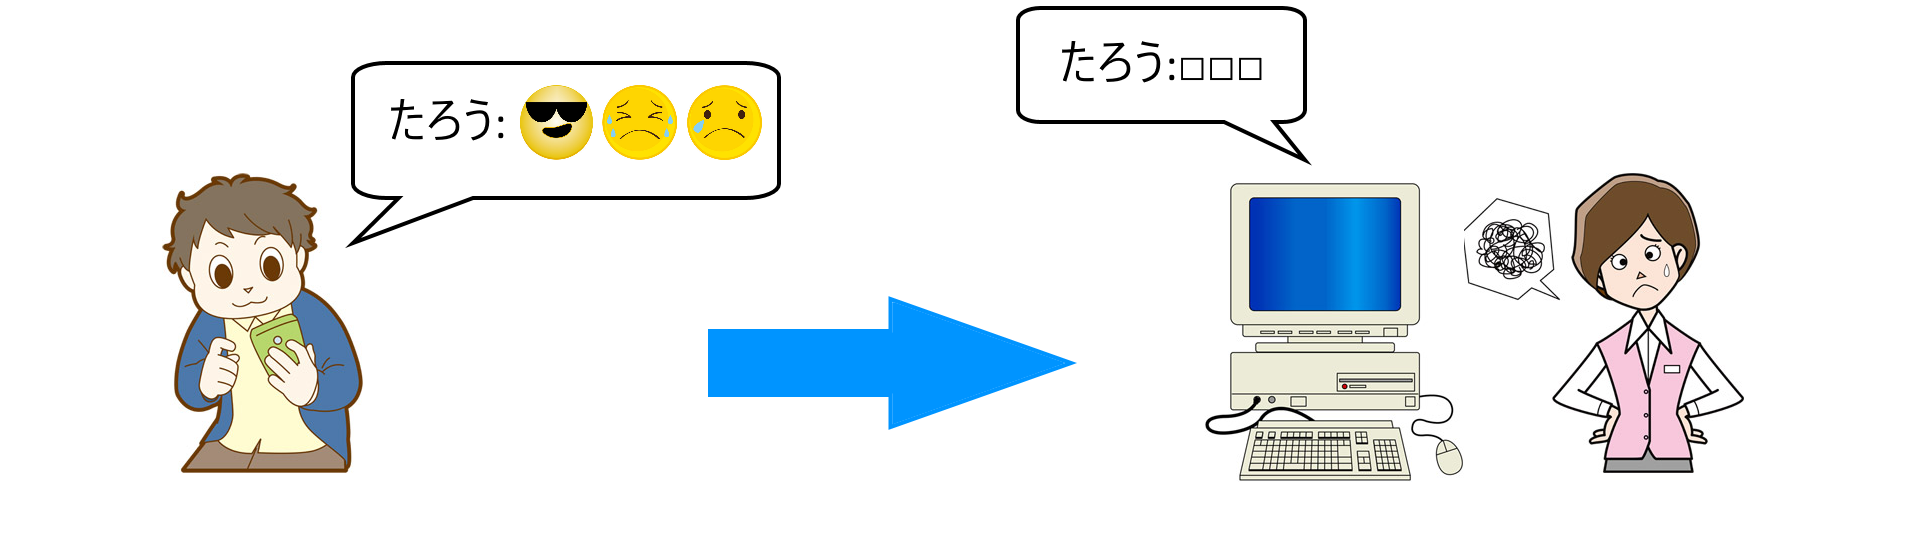
\includegraphics[width=\textwidth]{slide07-img/slide07-img005.png}}
            \end{minipage}
\end{frame}

\begin{frame}[fragile]
    \frametitle{ネチケットについて知ろう\\テキスト P.\pageref{1:P:Netiquette}~~~\raisebox{-3mm}{
\includegraphics[width=0.06\textwidth]{./slide07-img/raspberry.png}}}
    % \frametitle{ネチケットについて知ろう}
    \large\textbf{迷惑メールは見ない、送らない}
            \begin{itemize}\small
                \item 迷惑メールは、悪い人が色々な都合で出してくる怪しいメールのことです。
                怪しいリンクや知らないソフトウェアが貼り付けられたりすることがあり、それを
                見るとウイルスという悪いものが入ってくることがあります。
                \item また、チェーンメール(呪いのメールなど)は絶対に信じず他の人に送ってはいけません。         
            \end{itemize}
            \vfill
            
			\begin{minipage}{\textwidth}
                {\upshape
                  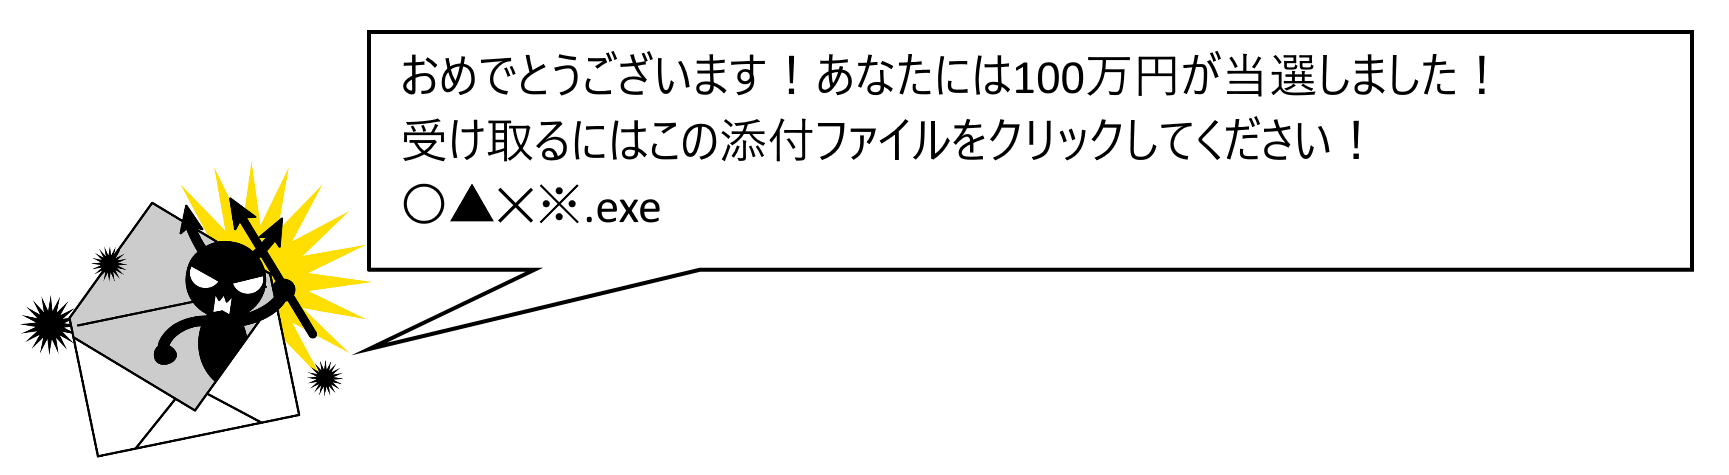
\includegraphics[width=\textwidth]{slide07-img/slide07-img006.png}}
            \end{minipage}
\end{frame}

\begin{frame}[fragile]
    \frametitle{ネチケットについて知ろう\\テキスト P.\pageref{1:P:Netiquette}~~~\raisebox{-3mm}{
\includegraphics[width=0.06\textwidth]{./slide07-img/raspberry.png}}}
    % \frametitle{ネチケットについて知ろう}
    \large\textbf{自分の情報を外に漏らさない}
            \begin{itemize}\small
                \item 自分の名前や、住所などをネットにあげるのはとても危ないから止めましょう。悪い人の
                目に入ってしまうと家族の身の危険にもつながり命の保証ができません。
                \item ネットに一度でもあげてしまうと消すことができなくなります。
            \end{itemize}
            \vfill
            
			\begin{minipage}{\textwidth}
                {\upshape
                  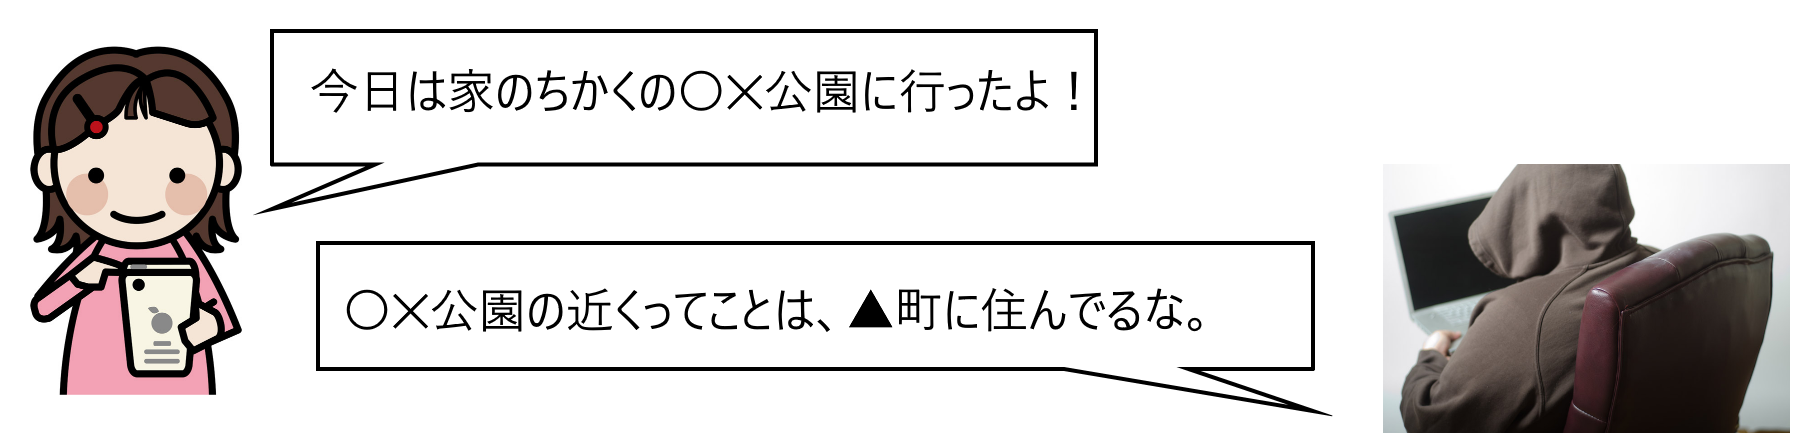
\includegraphics[width=\textwidth]{slide07-img/slide07-img007.png}}
            \end{minipage}
\end{frame}

\begin{frame}[fragile]
    % \frametitle{インターネットについて知ろう}
    \frametitle{インターネットについて知ろう\\テキスト P.\pageref{1:P:internet}~~~\raisebox{-3mm}{
\includegraphics[width=0.06\textwidth]{./slide07-img/raspberry.png}}}
		\begin{description}
			\item[ネットワーク] ~\\
				\begin{itemize}\small
					\item お互いの情報をこうかんできるようにしたもの
				\end{itemize}

			\item[インターネット]~\\
				\begin{itemize}\small
					\item ネットワークがお互いにつながりあい網の目のように世界中に広がっているそのもの
				\end{itemize}
		\end{description}
		\vfill
        \begin{minipage}{0.5\textwidth}
            {\upshape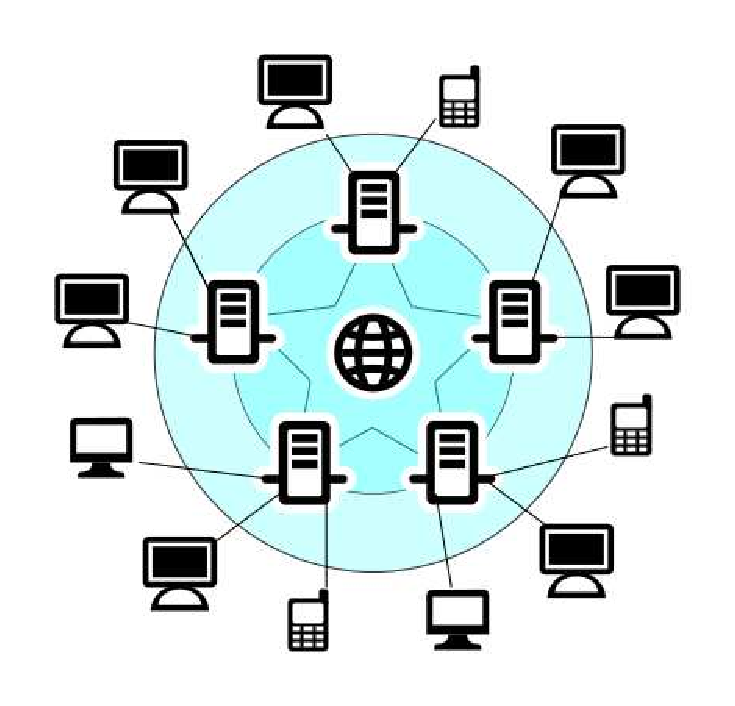
\includegraphics[scale=0.3]{text07-img/ome7-img002.eps}}
        \end{minipage}
\end{frame}

\begin{frame}[fragile]
	\frametitle{インターネットについて知ろう\\テキスト P.\pageref{1:P:internet}~~~\raisebox{-3mm}{
\includegraphics[width=0.06\textwidth]{./slide07-img/raspberry.png}}}
    % \frametitle{インターネットについて知ろう}  
    \large\textbf{教科書をよみながら、問題をやってみよう}
				\begin{itemize}\small
					\item \ref*{1:Q:internet} P.\pageref{1:Q:internet}
				\end{itemize}
      \vfill
      \large\textbf{わからないことは、放っておかず、すぐに TA に聞きましょう}
\end{frame}

\begin{frame}[fragile]
	\frametitle{\large{IPアドレスについてりかいしよう\\テキスト P.\pageref{1:P:IP}-P.\pageref{1:P:port}}~~~\raisebox{-3mm}{
\includegraphics[width=0.06\textwidth]{./slide07-img/raspberry.png}}}
    %  \frametitle{\large{IPアドレスについてりかいしよう}}
     \textbf{IPアドレスは、ネットワーク上のコンピュータの住所}
          \begin{itemize}\small
             \item IPアドレスは、xxx.xxx.xxx.xxxのように3ケタずつ「.」で区切った4つの数字で表します。xxxには0{\textasciitilde}255の数字が入ります
             \item IPアドレスを用いてデータの送受信先を特定するため、1つのネットワークに同じIPアドレスはありません。
         \end{itemize}
         \vfill
            
		\begin{minipage}{\textwidth}
             {\upshape
                % 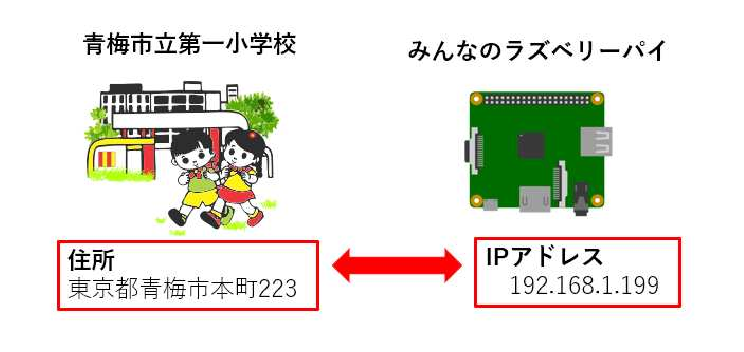
\includegraphics[width=\textwidth]{text07-img/ome7-img003}}
                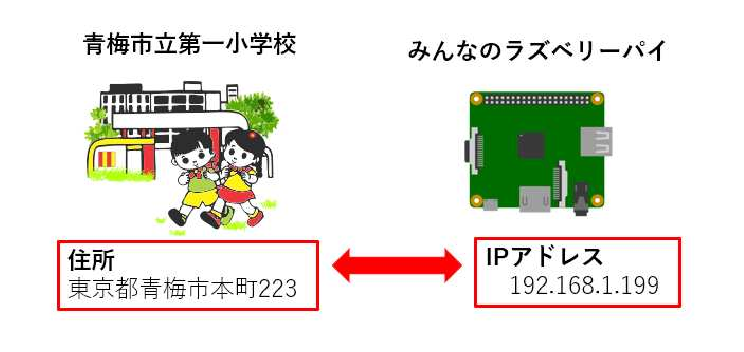
\includegraphics[scale=0.6]{text07-img/ome7-img003}}
        \end{minipage}
\end{frame}

\begin{frame}[fragile]
	\frametitle{\large{IPアドレスについてりかいしよう\\テキスト P.\pageref{1:P:slide_p12}}~~~\raisebox{-3mm}{
\includegraphics[width=0.06\textwidth]{./slide07-img/raspberry.png}}}
    % \frametitle{\large{IPアドレスについてりかいしよう}}
    \textbf{グローバルIPアドレスとローカルIPアドレス}
            \begin{itemize}\small
                \item IPアドレスは、インターネット上のコンピュータに割り当てられるグローバルIPアドレスと、内部ネットワーク上の各コンピュータに与えられるローカルIPアドレスの2種類があります。
            \end{itemize}
            \vfill
            
			\begin{minipage}{0.7\textwidth}
                {\upshape
                  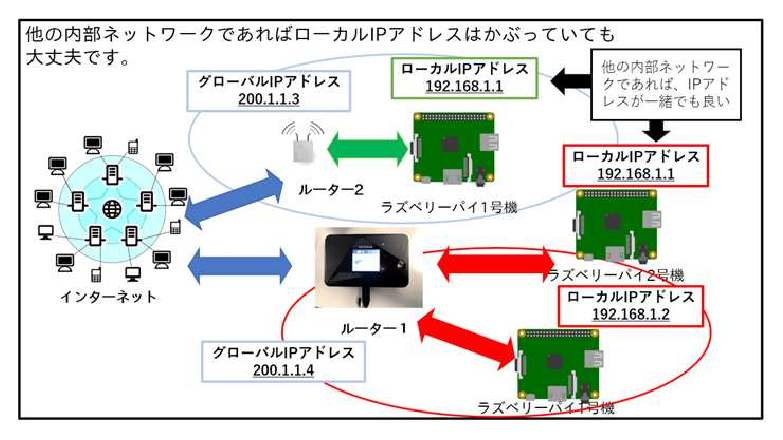
\includegraphics[width=\textwidth]{text07-img/ome7-img006}}
            \end{minipage}
\end{frame}

\begin{frame}[fragile]
	\frametitle{\large{IPアドレスについてりかいしよう\\テキスト P.\pageref{1:P:slide_p13}}~~~\raisebox{-3mm}{
\includegraphics[width=0.06\textwidth]{./slide07-img/raspberry.png}}}
    % \frametitle{\large{IPアドレスについてりかいしよう}}
    \large\textbf{教科書をよみながら、じゅんばんに問題をやってみよう}
				\begin{itemize}\small
					\item \ref*{1:Q:localIP} P.\pageref{1:Q:localIP}
					\item \ref*{1:E:checkIP} P.\pageref{1:E:checkIP}
				\end{itemize}
      \vfill
      \large\textbf{わからないことは、放っておかず、すぐに TA に聞きましょう}
\end{frame}

\begin{frame}[fragile]
	\frametitle{\large{IPアドレスについてりかいしよう\\テキスト P.\pageref{1:P:slide_p14}}~~~\raisebox{-3mm}{
\includegraphics[width=0.06\textwidth]{./slide07-img/raspberry.png}}}
            
    % \frametitle{\large{IPアドレスについてりかいしよう}}
    \begin{itemize}\small
                \item みなさんのラズベリーパイは直接インターネットにつながっているのではなく、グローバルIPアドレスをもつルータを通ってインターネットに接続しています
            \end{itemize}
            \vfill
            
			\begin{minipage}{\textwidth}
                {\upshape
                  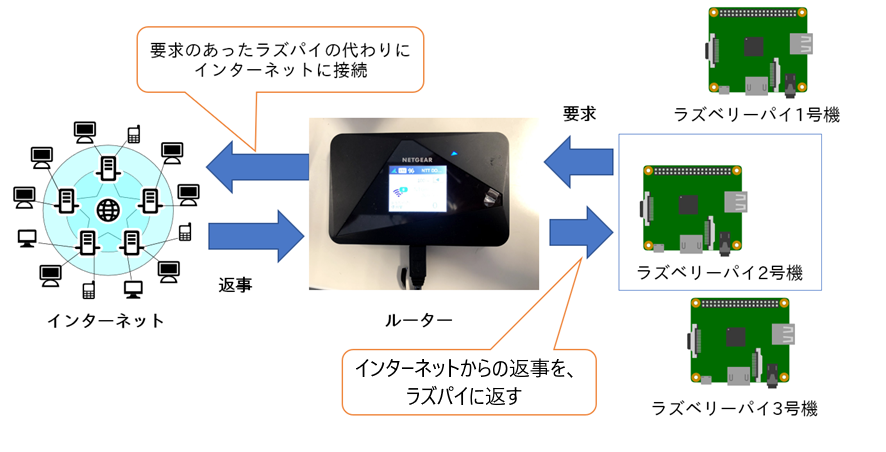
\includegraphics[width=\textwidth]{text07-img/ome7-img013.png}}
            \end{minipage}
\end{frame}

\begin{frame}[fragile]
	\frametitle{\large{IPアドレスについてりかいしよう\\テキスト P.\pageref{1:P:slide_p15}}~~~\raisebox{-3mm}{
\includegraphics[width=0.06\textwidth]{./slide07-img/raspberry.png}}}
    % \frametitle{\large{IPアドレスについてりかいしよう}}  
    \large\textbf{教科書をよみながら、じゅんばんに問題をやってみよう}
				\begin{itemize}\small
					\item \ref*{1:Q:globalIP} P.\pageref{1:Q:globalIP}
					\item \ref*{1:E:router} P.\pageref{1:E:router}
				\end{itemize}
      \vfill
      \large\textbf{わからないことは、放っておかず、すぐに TA に聞きましょう}
\end{frame}

\begin{frame}[fragile]
	\frametitle{\large{ポート番号についてりかいしよう\\テキスト P.\pageref{1:P:port}-P.\pageref{1:P:DNS}}~~~\raisebox{-3mm}{
\includegraphics[width=0.06\textwidth]{./slide07-img/raspberry.png}}}
    % \frametitle{\large{ポート番号についてりかいしよう}}        
    \begin{itemize}\small
                \item コンピュータでは多くのプログラムがネットワークを使用しています。そのため、IPアドレスだけでは、どのプログラムからと接続するのかを区別できません。
            \end{itemize}
            
			\begin{minipage}{\textwidth}
                {\upshape
                  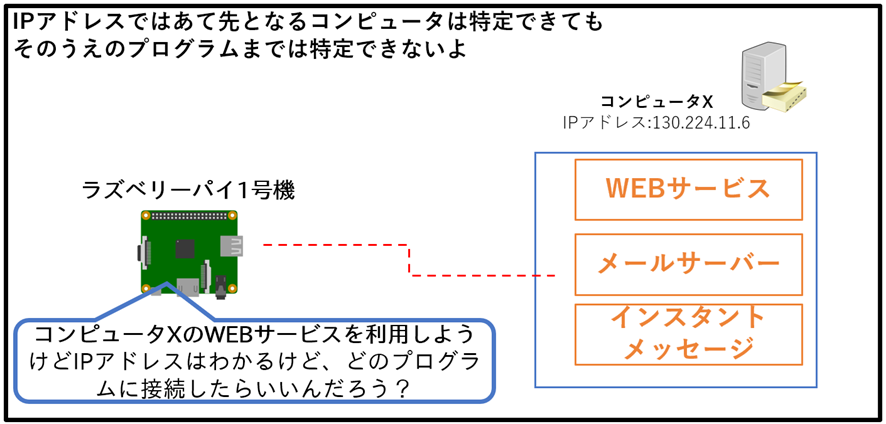
\includegraphics[width=\textwidth]{slide07-img/slide07-img011.png}}
            \end{minipage}
\end{frame}

\begin{frame}[fragile]
	\frametitle{\large{ポート番号についてりかいしよう\\テキスト P.\pageref{1:P:slide_p17}}~~~\raisebox{-3mm}{
\includegraphics[width=0.06\textwidth]{./slide07-img/raspberry.png}}}
    % \frametitle{\large{ポート番号についてりかいしよう}}        
    \begin{itemize}\small
                \item どのプログラムと接続するかを指定するためにポート番号が用いられます。
                \item ポート番号は、用途があらかじめ決まっている番号と、自由につかってよい番号の2種類があります。
            \end{itemize}
			\begin{minipage}{\textwidth}
                {\upshape
                  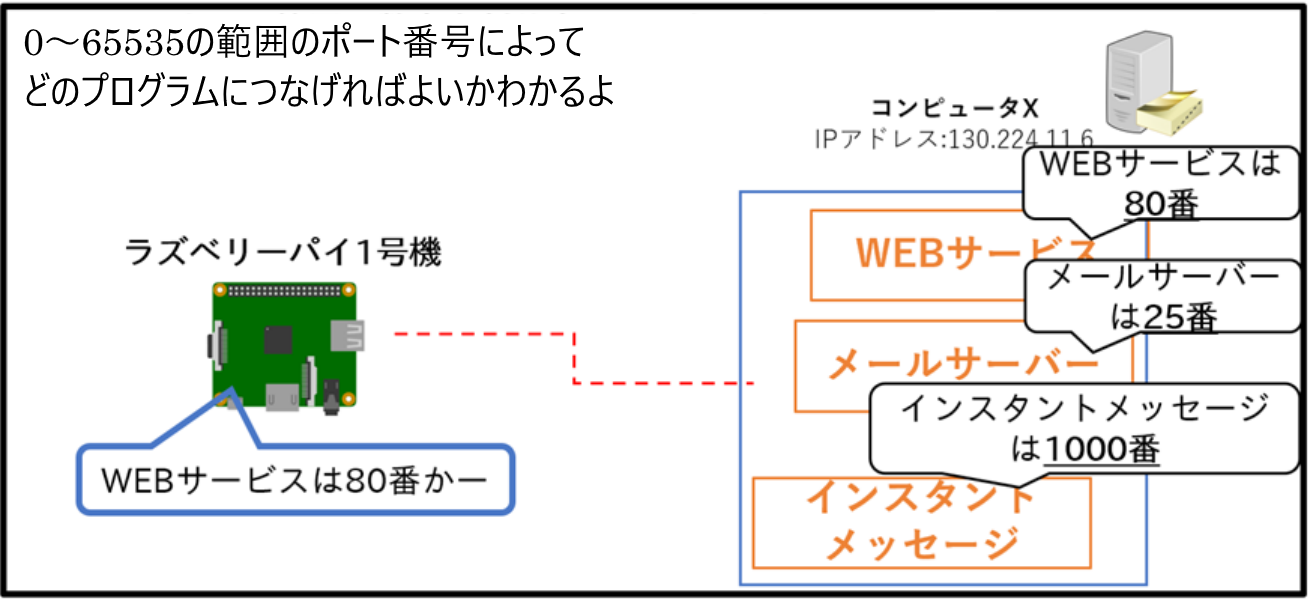
\includegraphics[width=\textwidth]{slide07-img/slide07-img012.png}}
            \end{minipage}
\end{frame}

\begin{frame}[fragile]
	\frametitle{\large{ポート番号についてりかいしよう\\テキスト P.\pageref{1:P:slide_p18}}~~~\raisebox{-3mm}{
\includegraphics[width=0.06\textwidth]{./slide07-img/raspberry.png}}}
    % \frametitle{\large{ポート番号についてりかいしよう}}        
    \begin{itemize}\small
                \item 受信側のポートは自動的に割り当てられます。
            \end{itemize}
			\begin{minipage}{\textwidth}
                {\upshape
                  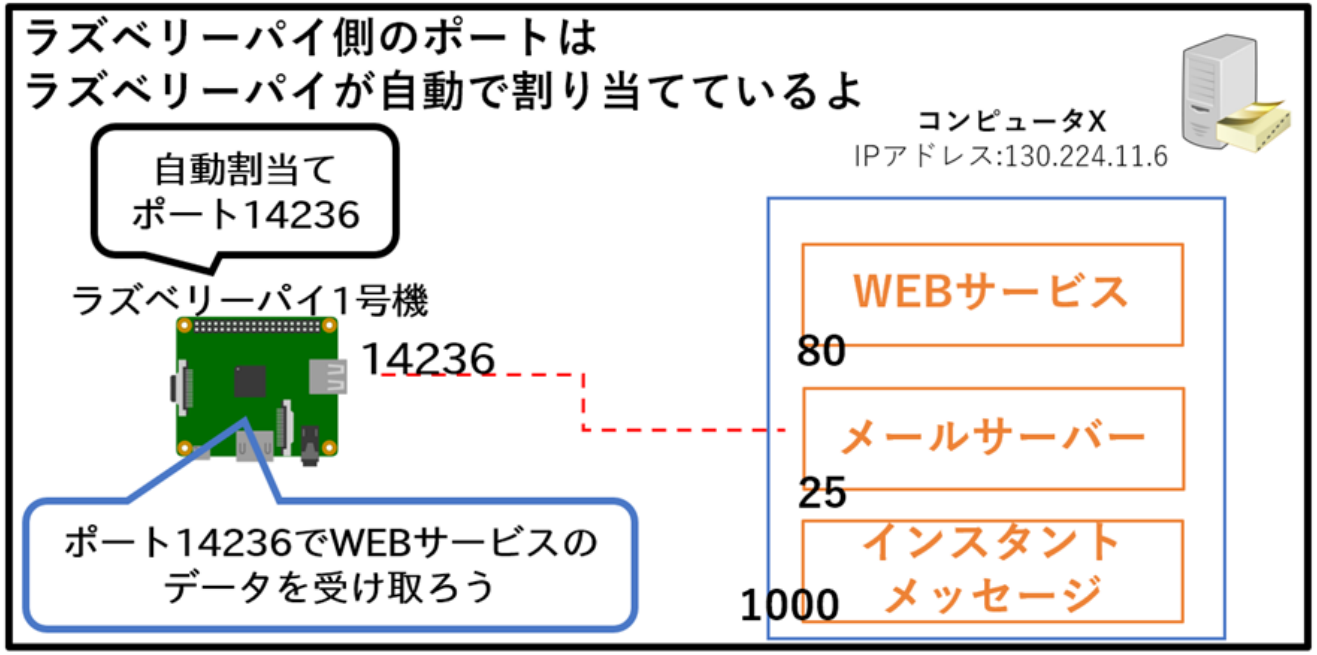
\includegraphics[width=\textwidth]{slide07-img/slide07-img013.png}}
            \end{minipage}
\end{frame}

\begin{frame}[fragile]
	\frametitle{DNSについてりかいしよう\\テキスト P.\pageref{1:P:DNS}~~~\raisebox{-3mm}{
\includegraphics[width=0.06\textwidth]{./slide07-img/raspberry.png}}}
    % \frametitle{DNSについてりかいしよう}        
    \begin{itemize}\small
                \item IPアドレスを知らないとサーバに接続することはできません。しかし、IPアドレスは人間にはわかりづらいです。
            \end{itemize}
			\begin{minipage}{\textwidth}
                {\upshape
                  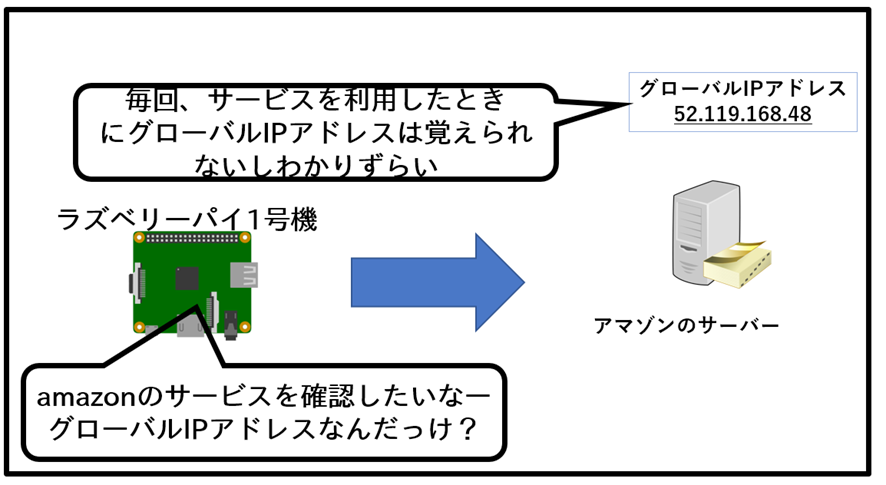
\includegraphics[width=\textwidth]{text07-img/ome7-img026.png}}
            \end{minipage}
\end{frame}

\begin{frame}[fragile]
	\frametitle{DNSについてりかいしよう\\テキスト P.\pageref{1:P:DNS}~~~\raisebox{-3mm}{
\includegraphics[width=0.06\textwidth]{./slide07-img/raspberry.png}}}
    % \frametitle{DNSについてりかいしよう}        
    \begin{itemize}\small
                \item IPアドレスとサーバの名前を対応づける、DNS(Domain Name System)という仕組みが使われています。
            \end{itemize}
			\begin{minipage}{\textwidth}
                {\upshape
                  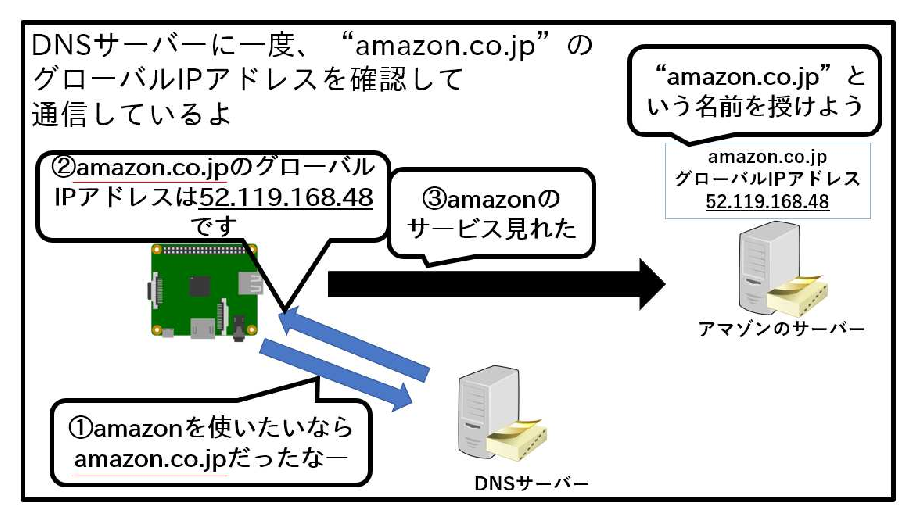
\includegraphics[width=\textwidth]{text07-img/ome7-img027}}
            \end{minipage}
\end{frame}




\begin{frame}[fragile]
	\frametitle{\large{ポート番号、DNSについてりかいしよう\\テキスト P.\pageref{1:P:port}-P.\pageref{1:P:HTML}}~~~\raisebox{-3mm}{
\includegraphics[width=0.06\textwidth]{./slide07-img/raspberry.png}}}
    % \frametitle{\large{ポート番号、DNSについてりかいしよう}}  
    \large\textbf{教科書をよみながら、じゅんばんに問題をやってみよう}
				\begin{itemize}\small
					\item \ref*{1:Q:portUsage} P.\pageref{1:Q:portUsage}
					\item \ref*{1:Q:port} P.\pageref{1:Q:port}
					\item \ref*{1:Q:dig} P.\pageref{1:Q:dig}
					\item \ref*{1:port} P.\pageref{1:port}
				\end{itemize}
      \vfill
      \large\textbf{わからないことは、放っておかず、すぐに TA に聞きましょう}
\end{frame}







